%Proofread by Dusan. Principalne OK. Tak volnejsie podane ale fajn.
Máme zmerať množstvo vody nasaté špagetami za nejaký čas pri nejakej teplote.
To znie ako niečo, čo bude trochu náročné na aparatúru, preto si treba najprv dobre premyslieť,
akým spôsobom to chceme merať a~či na to máme doma všetky potrebné veci.

Pod množstvom zo zadania úlohy môžeme rozumieť hmotnosť, ako aj objem vody.
Je na nás, aby sme sa zamysleli, čo z~toho chceme merať, teda na čo máme doma použiteľnú aparatúru a~vieme to zmerať jednoduchšie a~presnejšie.

Rozumný odmerný valec s~dostatočne malým najmenším dielikom na stupnici (aspoň \SI{1}{\centi\metre\cubed}) asi nemá doma každý.
Naproti tomu digitálna váha merajúca s~presnosťou na jeden gram rozhodne nie je v~domácnosti raritou, preto som osobne skôr za meranie hmotnosti než objemu. 

Ďalej budeme určite potrebovať kuchynský teplomer. Čím presnejší, tým lepšie. A~stopky. Alebo minútky. 

Keďže jedna časť úlohy vyžaduje držať špagety desať minút vo vode s~konštantnou teplotou, treba sa zamyslieť aj nad tým, ako tú teplotu udržať.
Možností je hneď niekoľko. Môžeme si zimprovizovať kalorimeter, ktorému budeme dôverovať natoľko, aby sme v~ňom tú vodu len tak nechali,
alebo použiť termohrnček, ktorému dostatočne dôverujeme, alebo stáť desať minút pri sporáku s~teplomerom strčeným v~hrnci a~podľa toho, ako sa teplota vody mení, ju prihrievať. Je to len na nás. 

Myslieť musíme aj na to, že sacia schopnosť sa podľa druhu špagiet môže líšiť, preto je fajn uviesť, aké špagety sme použili.

Keď máme vyriešenú aparatúru, môžeme pristúpiť k~samotnému meraniu. Prvá časť úlohy hovorí, že treba zistiť,
koľko vody nasajú špagety počas desiatich minút v~rôzne teplej vode. To neznie až tak zložito.
Navážime si špagety, zohrejeme vodu, celé to zavrieme do aparatúry a~odstopujeme si desať minút.
Potom špagety precedíme a~odvážime. Toto zopakujeme povedzme päťkrát pre päť rôznych teplôt
a~s~prvou časťou sme hotoví (samozrejme, čím viac teplôt odmeriame, tým lepšie budeme vedieť odhadnúť hľadanú závislosť). 

Druhá časť úlohy od nás chce, aby sme pre jednu teplotu zmerali závislosť množstva nasatej vody od času.
Teda si zvolíme nejakú teplotu, ktorá sa nám podľa prvého merania zdá najvhodnejšia, a~nejaký časový interval, po ktorom špagety zakaždým precedíme a~odvážime. 

Pri svojom meraní som použila termohrnček\footnote{Teplota v~ňom, sa počas merania menila maximálne o~pár stupňov Celzia, 
čo je rozhodne menej ako rozdiely medzi teplotami vody pri jednotlivých pokusoch},
historický teplomer s~najmenším dielikom $\SI{2}{\celsius}$,
digitálnu váhu merajúcu s~presnosťou na jeden gram a~bezvaječné špagety Clever. Pri prvom experimente bola počiatočná hmotnosť špagiet $\SI{19}{\gram}$, pri druhom $\SI{30}{\gram}$. Tu sú výsledky môjho merania:
\medskip

\begin{center}
\begin{tabular}{|c|c|c|}
\hline
  & $T$ \lbrack\si{\celsius}\rbrack & $\Delta m$ \lbrack\si{\gram}\rbrack \\
\hline
1. & 60   & 7   \\ \hline
2. & 70   & 11  \\ \hline
3. & 80   & 14  \\ \hline
4. & 90   & 19  \\ \hline
5. & 100  & 19  \\ \hline
\end{tabular}

\medskip

Tabuľka 1: Prírastky hmotnosti špagiet po desiatich minútach v~rôznych teplotách vody

\medskip

\begin{tabular}{|c|c|c|}
\hline
 & $t$ \lbrack\si{\second}\rbrack & $\Delta m$ \lbrack\si{\gram}\rbrack \\
\hline
1. & 120 & 15 \\ \hline
2. & 240 & 18 \\ \hline
3. & 360 & 22 \\ \hline
4. & 480 & 26 \\ \hline
5. & 600 & 30 \\ \hline
6. & 720 & 33 \\ \hline
7. & 840 & 36 \\ \hline
8. & 960 & 38 \\ \hline
9. & 1080 & 41 \\ \hline
10. & 1200 & 44 \\ \hline
\end{tabular}

\medskip


Tabuľka 2: Prírastky hmotnosti špagiet v~rôznom čase pri teplote $T = \SI{80}{\celsius}$

\end{center}

Odmerané máme, môžeme pristúpiť k~interpretácii údajov. Tu sa ujíma slova ľubovoľný tabuľkový editor. Mohli ste použiť {\it Excel}, {\it LibreOffice Calc},$\,$... Na vykreslenie grafov sme sa však rozhodli použiť {\it Gnuplot}.

Grafický výstup merania závislosti prírastku hmotnosti špagiet od teploty (prvá časť úlohy) by mohol vyzerať nejako takto: 

%Tu bude graf bez fitu
\begin{figure}[h]
\centering 
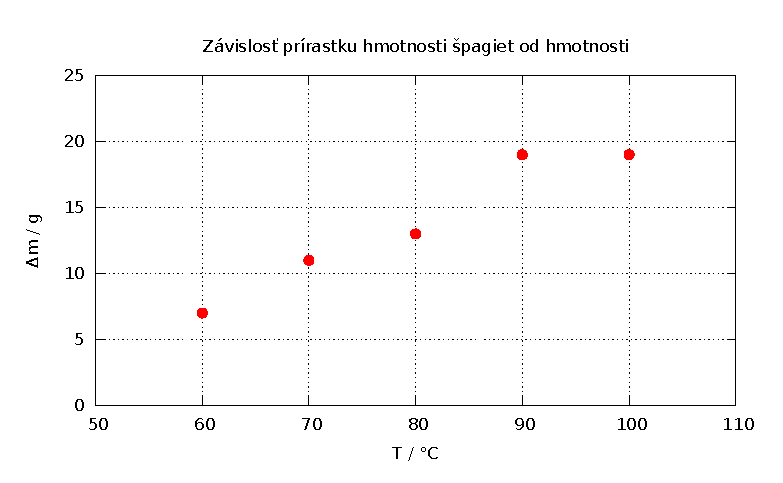
\includegraphics[scale=0.8]{graaf1.eps}
\caption{Grafické spracovanie prvého merania (Áno, nemám graf graf plný bodov, lebo som si povedala, že na ukážku to bude stačiť. Verím, že vy máte lepšie.)}
\end{figure}

\newpage
%Použijeme veľmi užitočnú fičúriu na zobrazenie trendovej čiary. Keďže vidíme, akým spôsobom nám hmotnosť rástla,
%dedukujeme, že daná závislosť sa najviac podobá na logaritmickú. Pomocou Excelu vieme zistiť aj koeficienty našej závislosti.

Druhé meranie nám poskytlo takýto výsledok:

\begin{figure}[h]
\centering
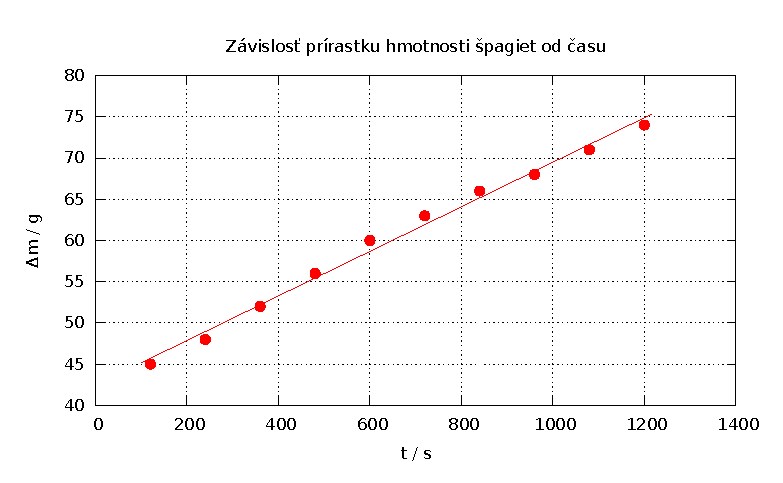
\includegraphics[scale=0.8]{graaf2.eps}
\caption{Grafické spracovanie druhého merania}
\end{figure}

%V~tomto prípade ide očividne o~lineárnu závislosť. Opäť vieme veľmi jednoducho zistiť jej koeficienty a~ak sme veľkí makači,
%pomocou funkcie LINEST\footnote{\url{http://www.colby.edu/chemistry/PChem/notes/linest.pdf}} vieme zistiť smerodajné odchýlky týchto koeficientov.

%Záver zmeníme podľa potreby.

Na záver nám zostáva zamyslieť sa, čo všetko nám mohlo spôsobiť nepresné meranie.
V~prvom rade to boli úniky tepla do okolia. V~kuchynských podmienkach sa ťažko vyrába dokonale izolovaná sústava. 
Pri použití termohrnčeka (malej termosky), tieto straty obmedzíme, no ako bolo spomenuté, teplota sa počas merania môže zmeniť
o~niekoľko stupňov.\footnote{Táto zmena bude určite menšia ako $\SI{10}{\celsius}$, čo sú rozdiely medzi nami 
meranými teplotami.} Okrem toho teplomer mal presnosť $\pm \SI{1}{\celsius}$, čo chyba rádovo na úrovni tých, čo spôsobili 
úniky tepla. 
Ďalšími meranými veličinami bol čas a hmotnosť špagiet. Nepresnosti stopiek a váhy sú dostačne malé na to, 
aby signifikantne prispievali k~chybám merania. No je tu ešte jedna vec, na ktorú nemôžeme zabudnúť, 
a to je dostatočné scedenie špagiet. Ak to neurobíme poriadne, nejaká voda nám tam zostane. Pokojne aj gram, či dva. 
Zdá sa to málo, ale keď sa zamyslíme nad tým, aké hmotnosti meriame, tak už i ten gram navyše nám spôsobí nepresnosť 
$5 - 10 \%$. Zvyšné zdroje, ako rozpúšťanie škrobu zo špagiet do vody, alebo odparovanie vody zo špagiet počas merania,
nemá zmysel uvažovať, lebo ich efekt je rádovo menši, ako tých pred chvíľou spomenutých.
až po nejakú tú hmotnosť navyše spôsobenú nedostatočným odkvapkaním scedených špagiet.

A~máme hotovo, môžeme ísť jesť. Keby mal niekto záujem o~recept na mega pseudobolonskú omáčku, ktorá je jednoduchá a~určite nesklame, napíšte mi ;).
